\section{Motivating example 1}
\label{sec:intro:me1}

With the univariate case (one observation variable $x$ and one response variable $y$), we generate and alter a sample of 100 data points from a normal distribution. We have developed this data to illustrate an interesting phenomenon. Even in this simplistic setting, numerical tools commonly used in regression analysis can fail dramatically when not accompanied by corresponding visualization tools.

For the purpose of this example, imagine that a data analyst cannot produce any plots in the analysis, and the desired question to answer is if $x$ contains explanatory power of $y$. The natural thing to try first is to fit simple linear regression and determine the significance of its coefficient. Doing this, the ANOVA table returns a significance level of 0.9109, extremely insignificant. When a constant-mean regression is performed, the resulting p value is equally as insignificant. The natural next step is to check the significance of each term in the linear regression model. Although the $x$-intercept ($0.460878, p < 2e-16$) is significantly non-zero, the observed variable x is not ($0.008261, p = 0.911$). Finally, a hypothesis test is used to determine whether or not the residuals are normally-distributed. The large $p$-value ($0.5795$) of the Shapiro test suggests it is. Next, one can check various correlations of $x$ against the residuals or $x$ against $y$, and each test yields no significant correlation. The raw data can be numerically printed out, but it's difficult to spot any trends in the data itself. Since there is little information that can gleaned on where to proceed next, it seems reasonable to conclude that the data is uncorrelated. The result is that the analyst scraps the regressions as they were ``uninteresting.''

Now assume that the analyst is allowed access to plotting tools in order to verify their numerical result. Once he/she plots the data (Figure~\ref{fig:intro:me1plot}), something peculiar happens. He/she finds that the analysis was completely incorrect. There is a strong $v$-shaped dependence between $x$ and $y$.  Nothing informed the analyst that there may be a nonlinear trend as none of the common hypothesis tests for linear regression failed, so the analyst would not suspect that the true trend was quadratic until the data was plotted. This example illustrates the fact that visualizations can lead to vastly different conclusions and act as a ``sanity check'' for the numerical results. 

\begin{figure}[htb]
	\begin{center}
		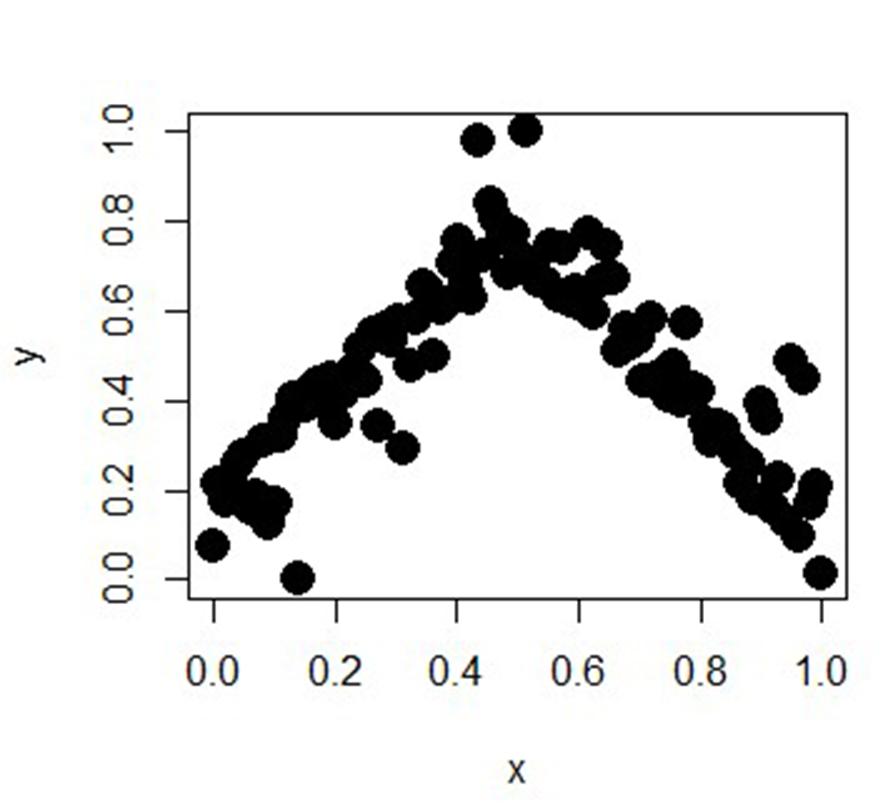
\includegraphics[width=0.5\linewidth]{ch-intro/figures/me1plot}
		\caption[A plot of data that exhibits a strong quadratic trend but fails common tests of dependence.]{A plot of data that exhibits a strong quadratic trend but fails common tests of dependence. The code for this analysis may be found in Appendix~\ref{sec:appendicies:me1plot}}
		\label{fig:intro:me1plot}
	\end{center}
\end{figure}